\section{Plots of Optimization Figure of Merit Components}
\label{sec:fomplots}

The figure of merit described in Equation~\ref{eq:fom} attempts to balance the
relative contributions of statistical sample size, sample purity, and sample
uncertainty to determine the optimal fiducial volume cuts. The plots in
Figure~\ref{fig:fom} show the total figure of merit that combines these three
factors.  In this section, we show plots of each of the constituent parts of
the figure of merit separately, which should demonstrate why the figure of
merit tends to favor certain FV cut regions.  Broadly speaking, the figure of
merit does not prefer large \towall and \wall cut values because this reduces
the total number of events (Figure~\ref{fig:nev}).  The figure of merit also
does not prefer small \towall and \wall cut values because this decreases
sample purity (Figure~\ref{fig:avgpow}) and/or sample uncertainty
(Figure~\ref{fig:avgsys}).  The ``optimal region'' lies somewhere between these
extremes.

\begin{figure}[h]
  \begin{center}
    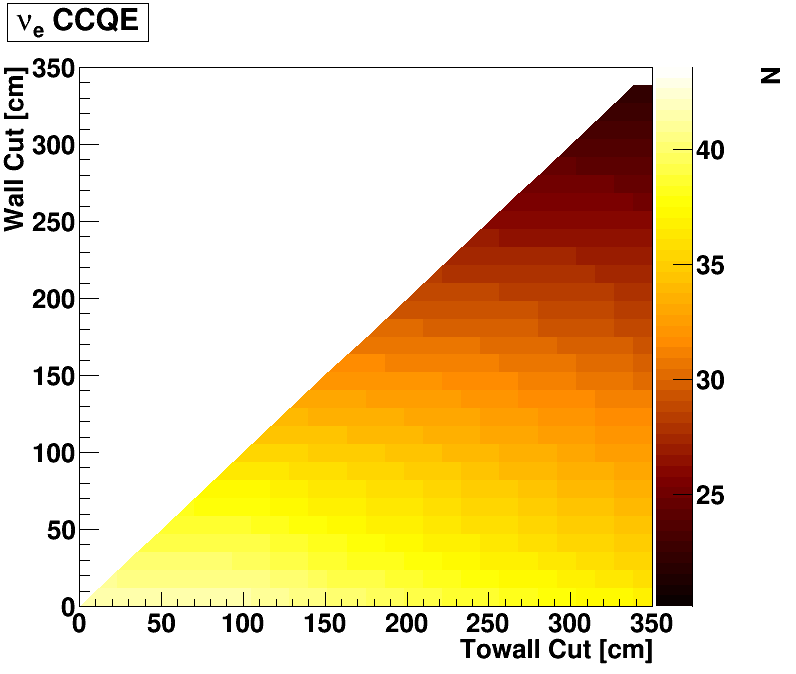
\includegraphics[width=0.45\textwidth]{fom_nev_nue}
    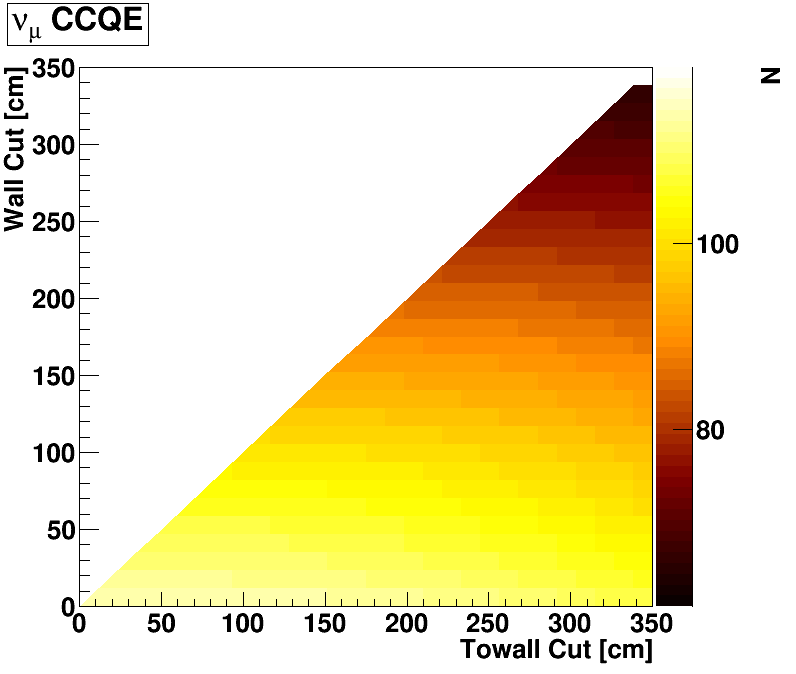
\includegraphics[width=0.45\textwidth]{fom_nev_numu}
    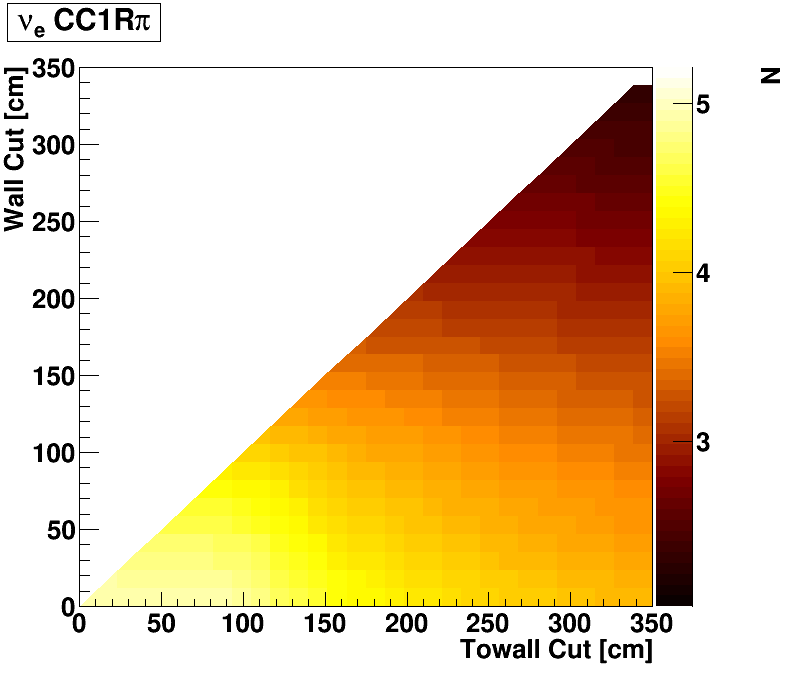
\includegraphics[width=0.45\textwidth]{fom_nev_nue1rpi}
  \end{center}
  \caption{Plots of the total expected number of events for each of the T2K
  event selections for various $(towall,wall)$ cut points.  As one would expect, smaller
  \towall and \wall cuts result in a larger overall sample size.}
  \label{fig:nev}
\end{figure}


\begin{figure}[h]
  \begin{center}
    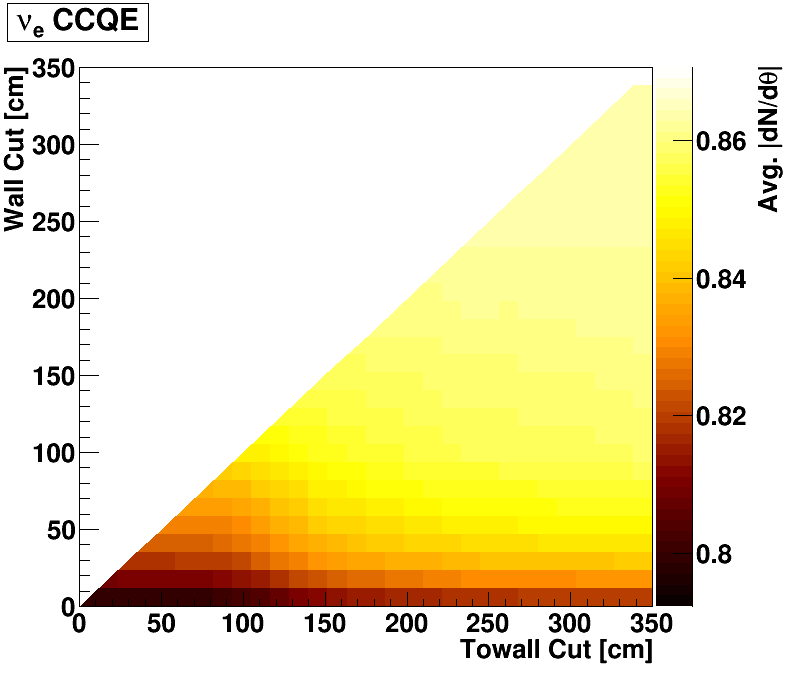
\includegraphics[width=0.45\textwidth]{fom_power_den_nue}
    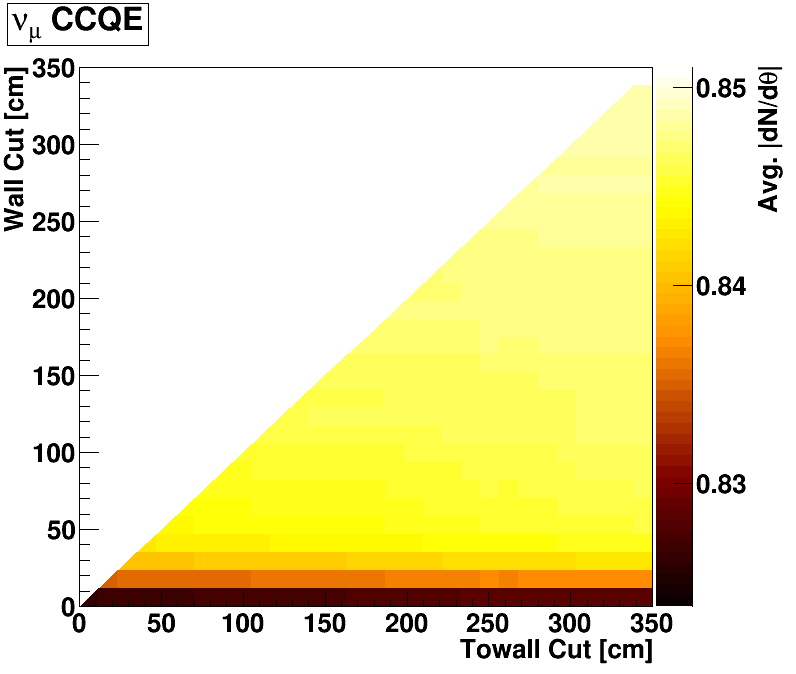
\includegraphics[width=0.45\textwidth]{fom_power_den_numu}
    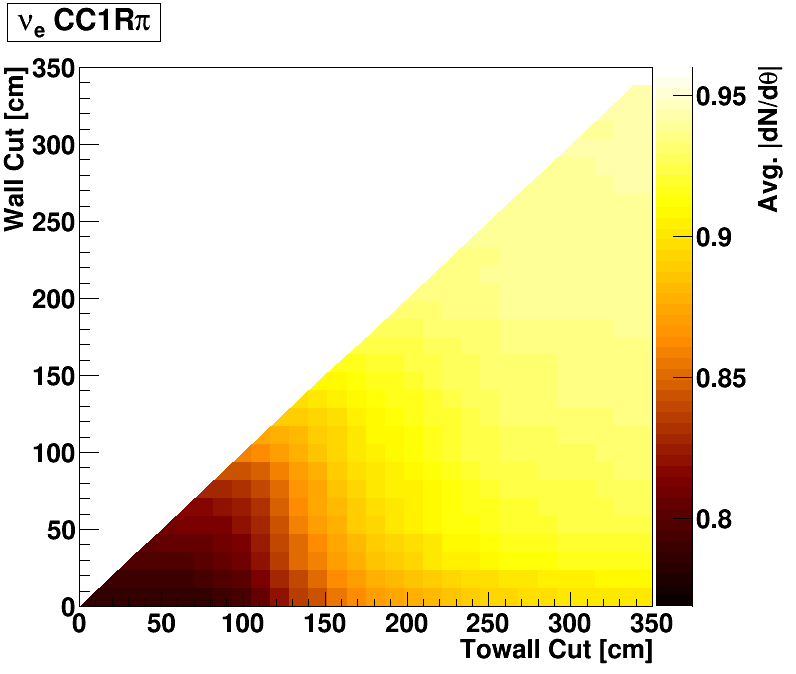
\includegraphics[width=0.45\textwidth]{fom_power_den_nue1rpi}
  \end{center}
  \caption{Plots of the average expected change in the number of events with
  respect to the oscillation parameter of interest at various $(towall,wall)$
  cut points and for each T2K event selection.  The contents of each bin shows
  the change in the number of events ($dN/d\theta$) for the FV cuts at that bin
  divided by the total number events ($N$) for that cut. The parameter $\theta$
  is \dcp for the \nue selections and \thdis for the \numu selections.  Darker
  regions denote degradation of the sample purity by adding ``background''
  events that contribute to $N$ but not $dN/d\theta$ (e.g.\@ neutral current
  events).}
  \label{fig:avgpow}
\end{figure}


\begin{figure}[h]
  \begin{center}
    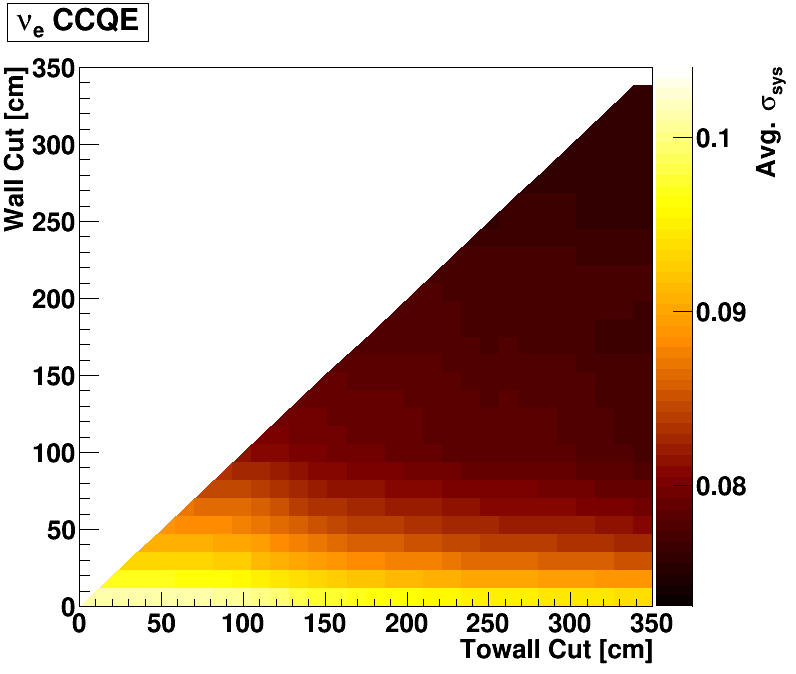
\includegraphics[width=0.45\textwidth]{fom_sys_den_nue}
    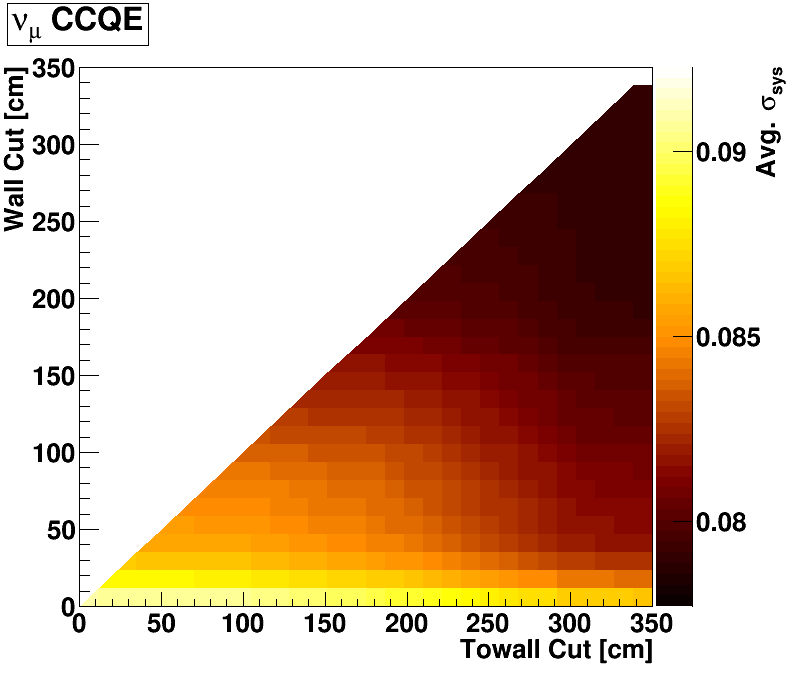
\includegraphics[width=0.45\textwidth]{fom_sys_den_numu}
    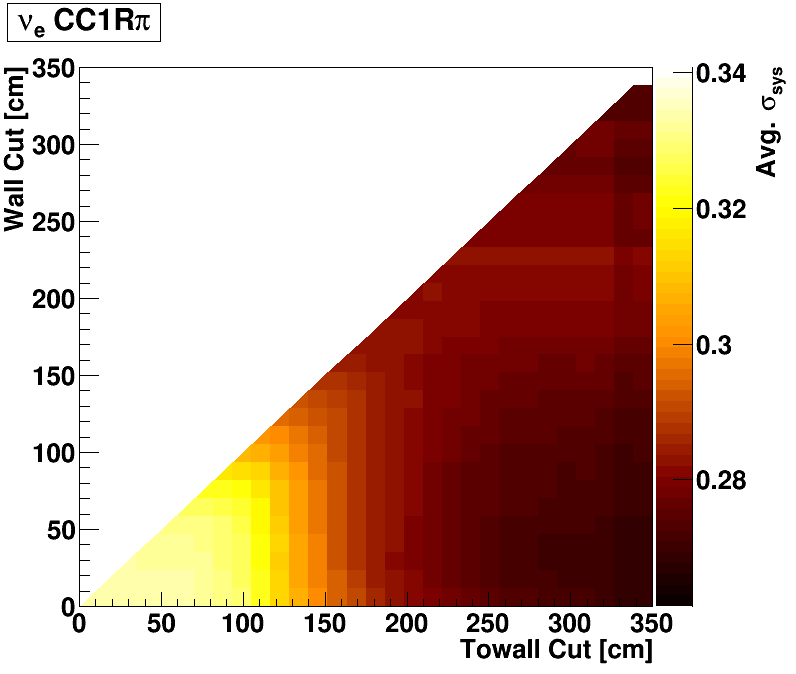
\includegraphics[width=0.45\textwidth]{fom_sys_den_nue1rpi}
  \end{center}
  \caption{Plots of the average overall systematic uncertainty estimate at various $(towall,wall)$
  cut points and for each T2K event selection.  Lighter regions denote a higher systematic uncertainty estimate,
  which arises from adding events with large uncertainty weights (e.g.\@ small \towall events, small \wall events, or
  entering events) to the sample.}
  \label{fig:avgsys}
\end{figure}



\FloatBarrier
